\chapter{Experiments and Discussion}
\label{ch:resultsAndAnalysis}

In this chapter we present how data is retrieved from social media,
what are the models we use for generating synthetic data and discuss the
results we obtain by running the methods presented in
\autoref{ch:solving}.

\section{Data collection and generation}%
\label{sec:data_collection_and_generation}

We now define techniques for generating synthetic data and present how real-world data is retrieved and preprocessed.

\subsection{Synthetic data}%
\label{sub:synthetic_data}

Here we propose two possible methods for generating data, the Signed SBM and
the Information spread model. Given $\tau \in \mathbb{N}$, both of these methods randomly generate
interaction graphs with $\tau$ threads/layers.
Depending on the method, they will require more parameters.

\subsubsection{Signed SBM}%
\label{ssub:signed_sbm}

This model is very similar to the Stochastic Block Model (SBM), a model
commonly used for generating random graphs having some community structures
\cite{Newman2018}.

The Signed SBM is based on the following parameters:
\begin{itemize}
	\item $k \in \mathbb{N}$, the number of communities.
	\item $b_{i} \in [k]$, the group assignment of each vertex $i$.
	\item $\omega ^{+} _{rs} \in [0, 1]$ and $\omega ^{-} _{rs} \in [0, 1]$, the probabilities
	      of positive and negative edges, respectively, between users in
	      group $r$ and $s$. Vertices have also a probability of not having an
	      edge, which is equal to $1 - \omega ^{-} _{rs} - \omega ^{+} _{rs} $.
	      For this reason it is needed that $\omega ^{+} _{rs} + \omega ^{-} _{rs} \leq 1$.
	\item $\theta \in [0, 1]$, controlling the reduction of the probability of interacting
	      between \emph{inactive} communities: for the generation of each
	      thread we will distinguish between \emph{active} and \emph{inactive}
	      communities, having different probabilities of interacting.
	\item $\hat{k} \in \mathbb{N}$, the number of communities active in
	      a thread.
\end{itemize}

During the generation process, we will sample the edges from a categorical
distribution with three parameters which we will denote as
\begin{equation*}
	\Omega = (\Omega^+, \Omega ^-, \Omega ^0).
\end{equation*}
$\Omega ^+$ and $\Omega ^-$ are the probabilities of adding a positive and
negative edges, respectively, while $\Omega ^0$ is the probability of not
adding any edge.

\bigskip

Therefore, generating a thread layer T\footnote{In this model we will generate
	contents uniquely associated to threads.} for an interaction graph
involves the following steps:
\begin{enumerate}
	\item Sample uniformly $\hat{k}$ of the $k$ communities. These are the
	      \emph{active} communities in the thread. The remaining communities
	      are \emph{inactive}.
	\item For each node pair $i, j$ consider their corresponding groups $r$ and
	      $s$ and, if both communities are \emph{active},
	      draw from
	      \begin{equation*}
		      \Omega = (\omega _{rs} ^{+}, \omega _{rs} ^{-}, 1 - \omega _{rs}
		      ^{+} - \omega _{rs} ^{-}).
	      \end{equation*}
	      Otherwise, if at least one of the
	      two communities is not \emph{active}, the distribution becomes
	      \begin{equation*}
		      \Omega = (\theta \omega _{rs} ^{+}, \theta \omega _{rs} ^{-}, 1 - \theta
		      (\omega _{rs} ^{+} + \omega _{rs} ^{-})).
	      \end{equation*}
	      Then, we possibly add the edge to thread $T$.

\end{enumerate}

\subsubsection{Information spread model}%
\label{ssub:information_spread_model}

Here we describe the Information spread model, which aims at simulating the
process of information flowing between different users of a social network.

Like in the Signed SBM, each node has a group assignment $b_i \in [k]$ and
each pair of groups has probabilities of
positive and negative edges ($\omega _{rs}^{+}  $ and $\omega _{rs}^{-}  $,
respectively, with $\omega ^{-} _{rs} + \omega ^{+} _{rs}
	\leq 1$).
Additionally, we have the following new parameters:

\begin{itemize}
	\item $\{\phi_{rs} \}$, the edge probabilities of a standard SBM. A standard SBM
	      takes as parameters a group assignment for each node (we will use
	      $b_i$) and the
	      probability of edge between each pair of communities (exactly $\{\phi_{rs} \}$), producing an
	      unweighted and undirected graph.

	      This model is used for generating a graph $G_f$, which we will call the \emph{friend} graph,
	      representing the friendship relationships between the users. We will
	      refer to neighbors in this graph as \emph{friends}.
	\item $\beta _a$, the probability that a node is initially activated: we
	      will distinguish between \emph{active} and \emph{inactive} nodes, that will have
	      different probabilities of interacting.
	\item $\beta _n$, the probability that an \emph{inactive} node is activated
	      from an \emph{active} friend.
\end{itemize}

\bigskip
After generating $G_f$ from an SBM with parameters $\{\phi_{rs} \}$, the
generation of each thread of an \emph{interaction graph} goes as
follows:

\begin{enumerate}
	\item Initialize all nodes as \emph{inactive}.
	\item Activate each vertex with probability $\beta_{a}  $.
	\item Active nodes activate their inactive friends with
	      probability $\beta_n$. This step is repeatedly each time a new user
	      is activated, until the network becomes stable.
	\item Similarly to the Signed SBM, if two nodes are both active, draw
	      from
	      \begin{equation*}
		      \Omega = (\omega _{rs} ^{+}, \omega _{rs} ^{-}, 1 - \omega _{rs} ^{+} -
		      \omega _{rs} ^{-})
	      \end{equation*}
	      for adding a positive, negative or no edge. If, instead, at least one
	      of them is not active, draw from
	      \begin{equation*}
		      \Omega = (\theta \omega _{rs} ^{+}, \theta \omega _{rs} ^{-}, 1
		      - \theta (\omega _{rs} ^{+} + \omega _{rs} ^{-})).
	      \end{equation*}
\end{enumerate}

\subsection{Collection and preprocessing}%
\label{sub:collection_and_preprocessing}

Datasets are built over two social medias:
Twitter\footnote{\url{twitter.com}} and Reddit\footnote{\url{www.reddit.com}}; the data
collection process, consequently, slightly differs between them.

\paragraph{Twitter.}%
\label{par:twitter-data}

Interaction graphs from Twitter are mainly built starting from the tweets
of profiles associated to well-known news sources, like The
New York Times or Fox News, that typically post links to their articles:
the set of shared URLs are the contents $\mathcal{C} $ of the corresponding interaction graph.

% Each time a user tweets one of these URLs (as in
% \autoref{fig:twitter-thread}) this
% will create another thread related to the same content, and all the
% replies it receives will be part of this new thread. More specifically,
% consider

Each content $C \in \mathcal{C}$ will be represented just by its URL,
e.g.

	{\footnotesize
		\begin{center}
			\url{https://www.nytimes.com/2021/03/04/us/richard-barnett-pelosi-tantrum.html}.
		\end{center}
	}

Then, in order to find all threads related to $C$, we search Twitter for
the content URL to obtain the tweets containing it. Each of these tweets
will correspond to a different thread.

\medskip

In order to validate our methods, we also construct datasets in which users are labeled either as
\emph{democrat} or \emph{republican} \footnotemark. This is done by looking at the people a
certain user $v_i$ follows: for each account $v_j$ followed by $v_i$, if $v_j$ is a political representative, then we can
retrieve from Wikipedia the party to which $v_j$ belongs to (see, for
example, \autoref{fig:tex/img/wikipedia-elected}). Then, user $v_i$ is assigned a
label according to the party of the majority of the users $v_j$ this
follows.

Twitter data is retrieved with the help of Tweepy \cite{tweepy}, a Python
library for accessing the Twitter API, which has been patched for using some
features available only in the beta of the new v2 Twitter API.

\footnotetext{We choose these two labels since the news sources we analyze for this purpose are based in U.S.
	Also, we think political discussion are a main source of controversial
	content and so it is an interesting criterion according to which users
	can be differentiated.}

\begin{figure}
	\centering
	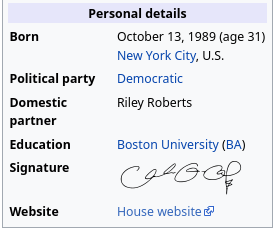
\includegraphics[width=0.4\linewidth]{tex/img/wikipedia-elected.png}
	\caption[Example Wikipedia entry]{Wikipedia entry associated to Alexandria Ocasio-Cortez, a member
		of the U.S. House of Representatives.}%
	\label{fig:tex/img/wikipedia-elected}
\end{figure}

\paragraph{Reddit.}%
\label{par:reddit}

Differently from Twitter, Reddit focuses on subreddits, which are pages
collecting posts of users about a specific topic (e.g.\ r/politics,
r/economics, $\dots$). This means that
in the datasets built from this social media the contents $\mathcal{C} $ is the
set of URLs posted on these pages, which, differently from how we fetch data
from Twitter, most likely
come from different sources.

These posts are in turn \emph{crossposted}, i.e.\ reposted on other subreddits. Each of
these \emph{crossposts} will correspond to another thread.

We also analyzed a
very specific case, that of r/asktrumpsupporters. This subreddit is a "Q\&A
subreddit to understand Trump supporters, their views, and the reasons behind
those views. Debates are discouraged" (from its description). We found it interesting as it provides an explicit labeling of the
users who, before commenting in any of these posts, must "declare" their side
by choosing a \emph{flair}, which is shown next to the username of the person
commenting.  Three flairs are available: \emph{Trump Supporter}, \emph{Non
	supporter} and \emph{Undecided}.

The PRAW library is used for retrieving Reddit data \cite{praw}.

\paragraph{Edge weights assignment.}%
\label{par:assigning_edge_weights}

Once the threads interactions are retrieved, they are passed to a state-of-the-art
sentiment analyzer which labels them. More specifically, the model used is
RoBERTa, adapted and retrained for dealing with Twitter
data \cite{Barbieri2020}. The model is made available by the Transformers
python library \cite{wolf-etal-2020-transformers}.

The model, given a string of text, returns a probability distribution

\begin{equation*}
	(p_{neg}, p_{neu}, p_{pos})
\end{equation*}

whose parameters represent the probabilities of negative,
neutral and positive sentiment. Let
\begin{align}
	\label{eq:}
	p_n & \coloneqq p_{neg}, & p_p & \coloneqq p_{pos} + p_{neu}.
\end{align}
If $p_p > p_n $ we assign the edge weight $p_p$, otherwise $-p_n$.

% \bigskip
%
% Finally, complying with the current privacy legislation, all the data related
% to the user is pseudo-anonymized (accounts identifier are replaced by random
% ones) while no data is publicly available.

\paragraph{Initial observations on the datasets.}
\label{sub:some_observations_on_the_datasets}
Reddit and Twitter are intrinsically different social medias. As mentioned
before, Reddit focuses on subreddits, where all the discussions related to a
certain topic find their place and most of the users interested in the
theme gather. We think that this contributes to create community of users which are more
active and more likely to discuss among each other, as they end up looking at the
same posts and discussions.

Twitter, instead, is a much less "centralized" social media where there a lot
of \emph{hubs} (users with many followers) that discuss very similar topics but
have disjoint communities.
Think, as an example, to the Twitter accounts of Joe Biden and Donald Trump. We expect that
most of the followers of the first one are not followers of the latter, and
viceversa, even if both of them discuss U.S. politics. This means that many
users, even if they are interested in the same theme (U.S. politics in our example)
will rarely interact between each other.

The "centralization" of Reddit produces, in our data model, contents that are
associated with few threads. We observed that even the most discussed articles
on r/politics (a subreddit focusing on U.S.\ politics discussions) are
\emph{crossposted} only one to five times (see, for example,
\autoref{fig:tex/img/reddit-crossposts}), while on Twitter articles of the New York Times are
often shared even 100 times.

\begin{figure}
	\centering
	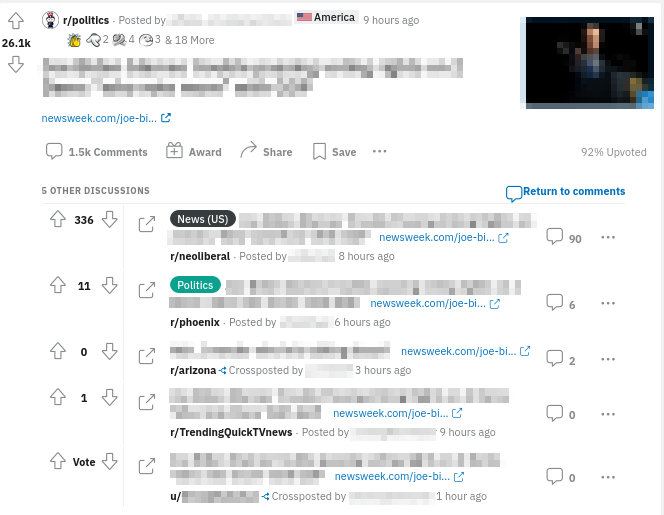
\includegraphics[width=0.8\linewidth]{tex/img/reddit-crossposts.png}
	\caption{The \emph{crossposts} on one of the most discussed article of the
		day on r/politics.}%
	\label{fig:tex/img/reddit-crossposts}
\end{figure}

\subsection{A study on r/asktrumpsupporters}%
\label{sec:the_r_asktrumpsupporters_case}

During the research we studied the r/asktrumpsupporters subreddit to
understand if it is possible to infer the community\footnotemark of the users by
looking at how they react to contents. More specifically, in a highly polarized
environment we expect that members in the same community of the
author have a positive stance towards the content; conversely, members of the
other communities have a negative one.

\footnotetext{In this case, we refer to community as the set of users with the same \emph{flair}}

\bigskip

For this analysis we add to our interaction graph another type of vertices, the
\emph{content nodes} which we uniquely associate to a content. More formally,
for each content $C \in \mathcal{C} $, we add a vertex $v_C$. In order to
add links between users and contents, we consider the sequence of comments
leading to a specific user comment and multiply the sign of the
associated edges to calculate the sign of the content-user edge.

For example, consider a user $v_i$
replying positively to a post related to content $C$ and user $v_j$ replying
negatively to $v_i$. We will add a positive edge between $v_i$ and $v_C$ and a
negative edge between $v_j$ and $v_C$.

We then assign to the users linked to a content the same label of the author of
the post if the user is connected to the content
by a positive edge and the opposite one\footnotemark otherwise. Then, we measure the accuracy of
this classification.

\footnotetext{We ignore the \emph{Undecided} label}

We show in \autoref{fig:tex/out/experimental200/experimental200-accuracy-hist}
the histogram of the accuracy of classification of the contents in the dataset.
We see that in very few cases it is possible to discriminate users better than
by just using the majority label ($79\%$), while a big part of the contents
achieve an accuracy between $0.5$ and $0.6$.

\begin{figure}
	\centering
	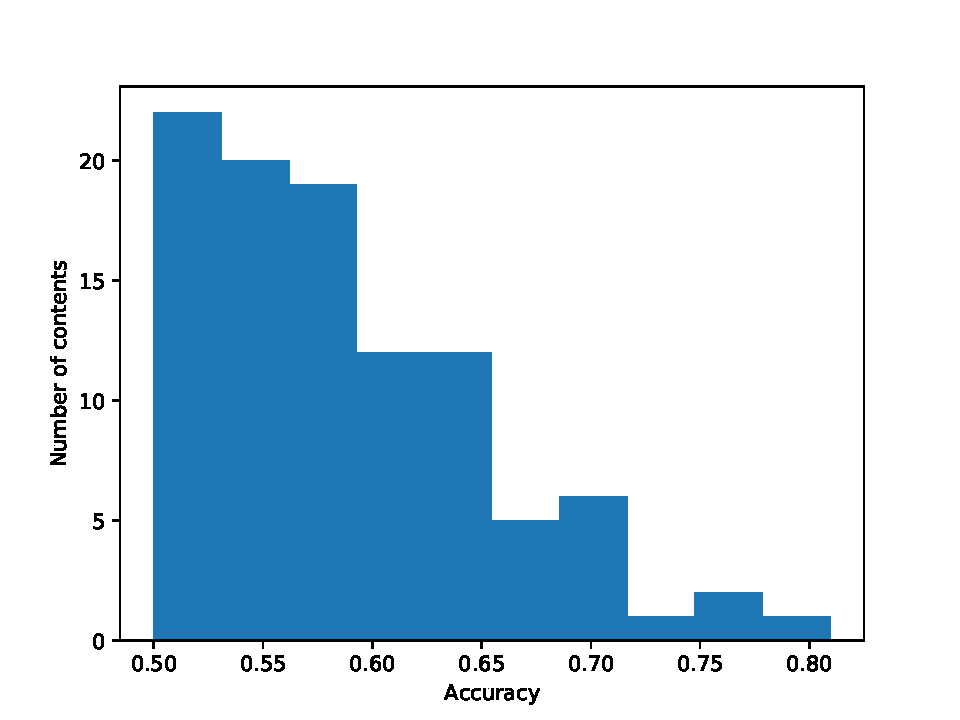
\includegraphics[width=0.6\linewidth]{tex/out/experimental200/experimental200-accuracy-hist.pdf}
	\caption[Distribution of accuracy of classification of r/asktrumpsupporters users for the
		different contents]{This plot shows how the accuracy of the classification
		process explained in \autoref{sec:the_r_asktrumpsupporters_case} is
		distributed for the different contents $C \in \mathcal{C} $. The graph
		used for the analysis contains $1850$ user vertices and
		$16470$ edges between them. Furthermore, there are $71$ content nodes
		and $5773$ content-user edges.}%
	\label{fig:tex/out/experimental200/experimental200-accuracy-hist}
\end{figure}

We explain this with the following reasons:
\begin{itemize}
	\item The majority of the posts in the subreddit are open questions, e.g.\ ``What
	      do you think of ...' and, similarly, ``What's your idea on...''. This
	      means that our initial hypothesis that positive and negative
	      stances can be used for inferring the positions of
	      the users is not correct: for this type of posts, and thus most of the users
	      will just answer with their opinion, without being either friendly or
	      hostile.
	\item This community of users is not a representative sample: people attending
	      the subreddit are open to discuss with people of different opinion
	      and for this reason we generally expect less hostility in the
	      comments.
\end{itemize}
\section{Experiments}

The following presented results have been obtained from a Python
implementation of the methods described in the previous chapters. The library used
for handling and manipulating graphs is graph-tool, which has been chosen
because of its efficiency \cite{peixoto_graph-tool_2014}.

\subsection{Initial real-world data analysis}%
\label{sub:validity_problem_definition}

We did an initial analysis of the data to understand basic properties of the
real-world datasets we fetched.

We can gain some insights about the existence of echo chambers by comparing
the distribution of $\eta(C)$ and $\eta(T)$ for different interaction graphs.
% Threads with an high fraction of positive edges may correspond to echo
% chambers, i.e. users that discuss a topic with no \emph{controversy}.
% Consequently, if we find an increase in the relative number of threads with a
% low $\eta(T)$ (with respect to content distribution) this may mean that this
% effect is already visible.
Intuitively, echo chambers may correspond to threads with a
high fraction of positive edges. Consequently, given a certain $\eta(C)$
distribution for the interaction graph, in presence of Echo Chambers we expect
an increase for low values of $\eta(T)$, when compared to the distribution of
$\eta(C)$.

We report these results for
three datasets, a first built over @nytimes, a second over @foxnews
and a third one over @bbcnews Twitter accounts\footnotemark. The basic
statistics of these graphs are listed in \autoref{tab:basic-statistics}. Histograms, obtained
by distributing values in $10$ equal-sized buckets, are shown in \autoref{fig:eta-content-thread}.

\footnotetext{As explained above (\autoref{sub:collection_and_preprocessing}), we are referring
	to the accounts that are used to retrieve the contents of the graph.}

By looking at these plots it is evident, as we were expecting, that when
moving from
contents to threads there is a significant increase in the percentage of
threads with a very small $\eta$, meaning that it is possible that contents which
globally have
a non-negligible amount of negative edges produce also threads that have
very few or no negative edges. These are the subgraphs in which we expect to
find the echo chambers. This is especially evident in the @nytimes and @bbcnews
datasets, while in @foxnews this effect is less visible.

\begin{table}
	\centering
	\caption{Basic statistics for analyzed datasets. Threads with no replies
		are excluded from the counts.}
	\label{tab:basic-statistics}
	\begin{tabular}{|c c c c c c|}
		\toprule
		Dataset  & $|V|$ & $|E|$  & $|\mathcal{C} |$ & Threads & Fraction of
		neg. edges                                                                         \\
		\midrule
		@foxnews & 45509 & 82494  & 311              & 1922    & \num{0.5884306737459694}  \\
		@nytimes & 81318 & 118876 & 492              & 6246    & \num{0.46229684713482955} \\
		@bbcnews & 16875 & 26636  & 380              & 1566    & \num{0.4381288481754017}  \\
		\bottomrule
	\end{tabular}
\end{table}

\begin{figure}
	\begin{center}
		\begin{subfigure}[b]{0.4\textwidth}
			\centering
			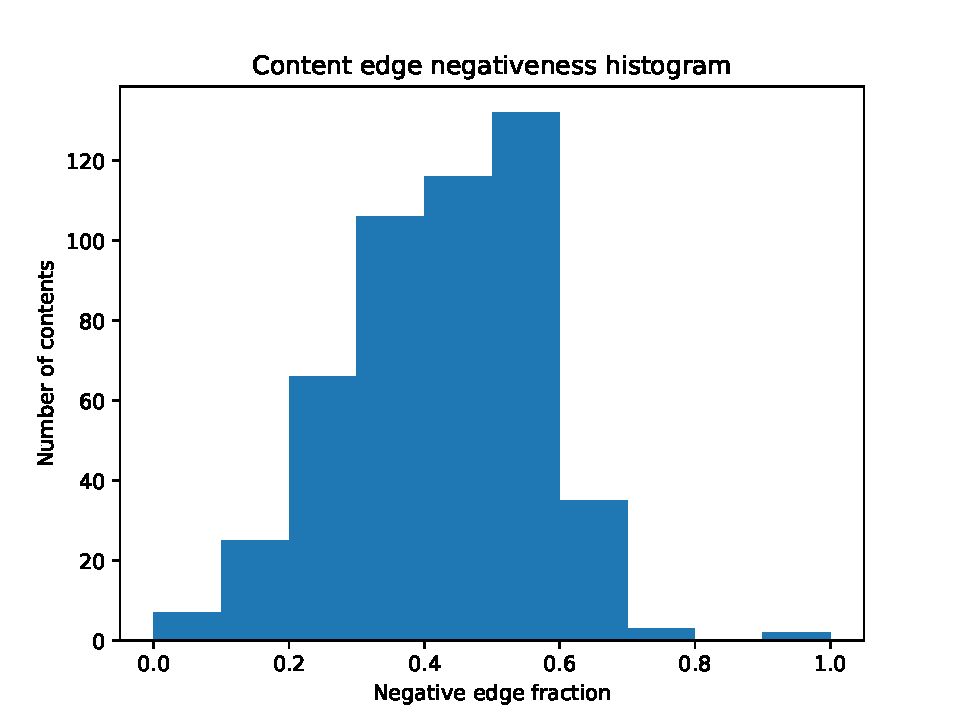
\includegraphics[width=\textwidth]{tex/out/nytimes700/neg-fraction-content-hist.pdf}
			\caption{$\eta(C)$ of @nytimes}
			\label{fig:nytimes-content-eta}
		\end{subfigure}
		\begin{subfigure}[b]{0.4\textwidth}
			\centering
			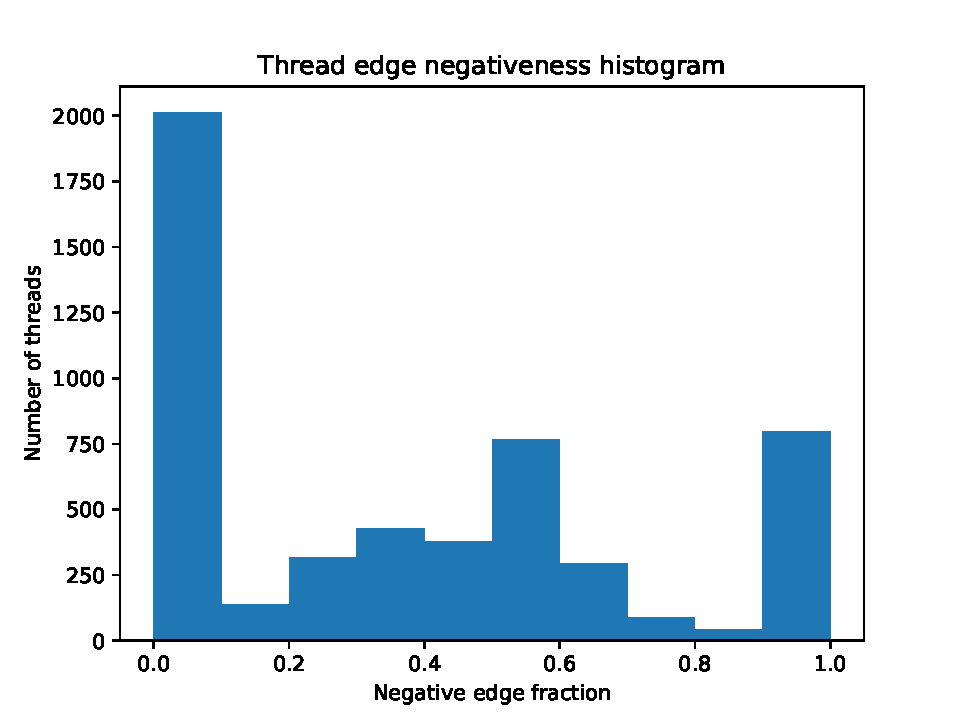
\includegraphics[width=\textwidth]{tex/out/nytimes700/neg-fraction-thread-hist.pdf}
			\caption{$\eta(T)$ for @nytimes}
			\label{fig:nytimes-thread-eta}
		\end{subfigure}
		\begin{subfigure}[b]{0.4\textwidth}
			\centering
			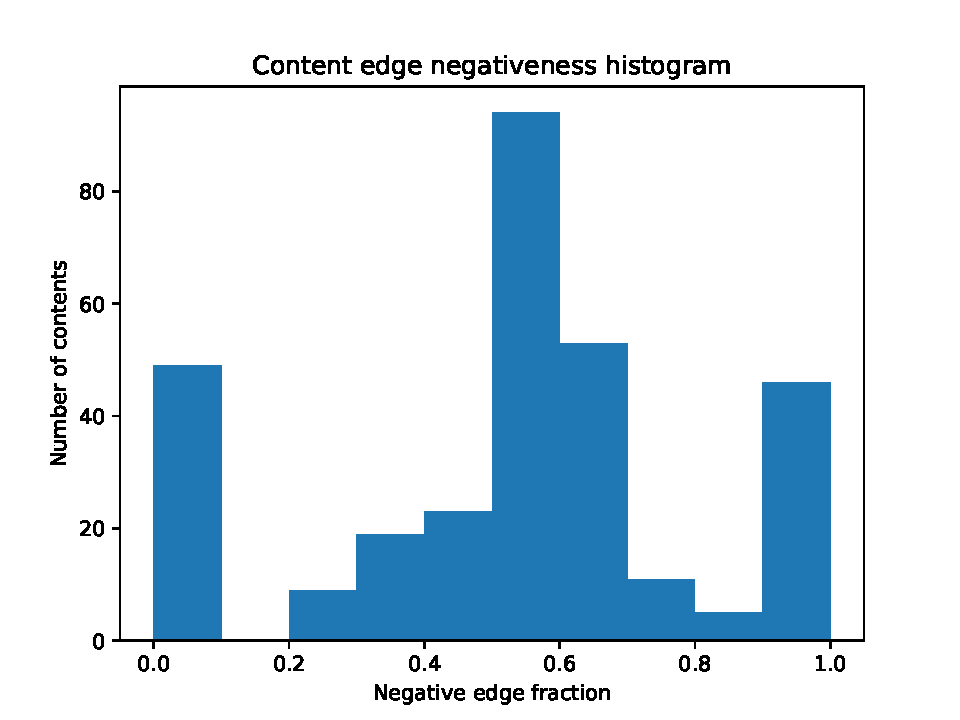
\includegraphics[width=\textwidth]{tex/out/foxnews2000/neg-fraction-content-hist.pdf}
			\caption{$\eta(C)$ of @foxnews}
			\label{fig:foxnews-content-eta}
		\end{subfigure}
		\begin{subfigure}[b]{0.4\textwidth}
			\centering
			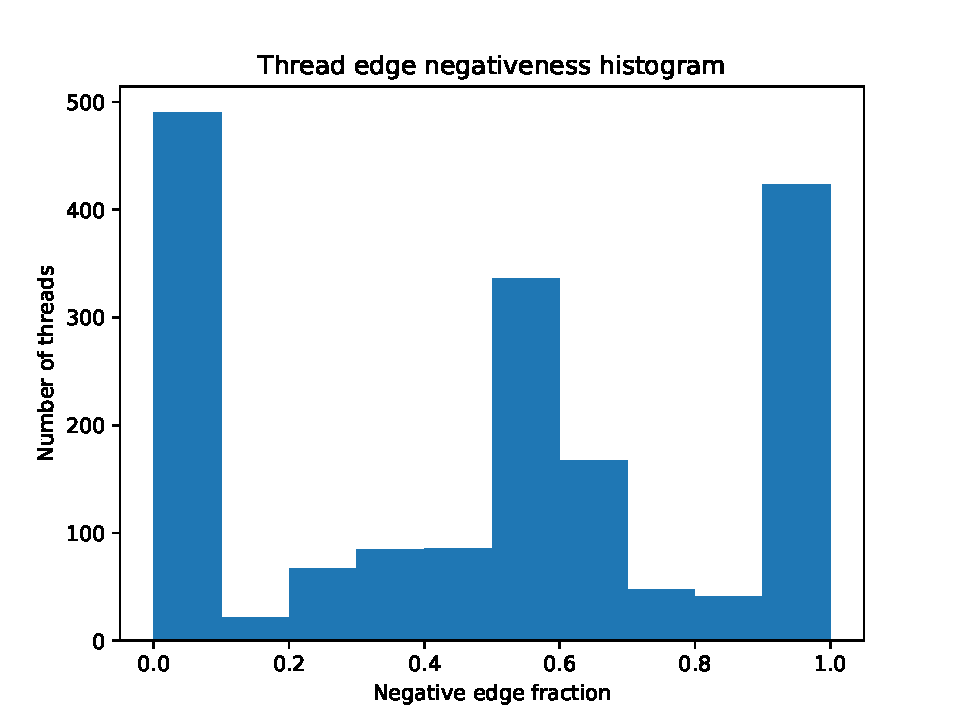
\includegraphics[width=\textwidth]{tex/out/foxnews2000/neg-fraction-thread-hist.pdf}
			\caption{$\eta(T)$ for @foxnews}
			\label{fig:foxnews-thread-eta}
		\end{subfigure}
		\begin{subfigure}[b]{0.4\textwidth}
			\centering
			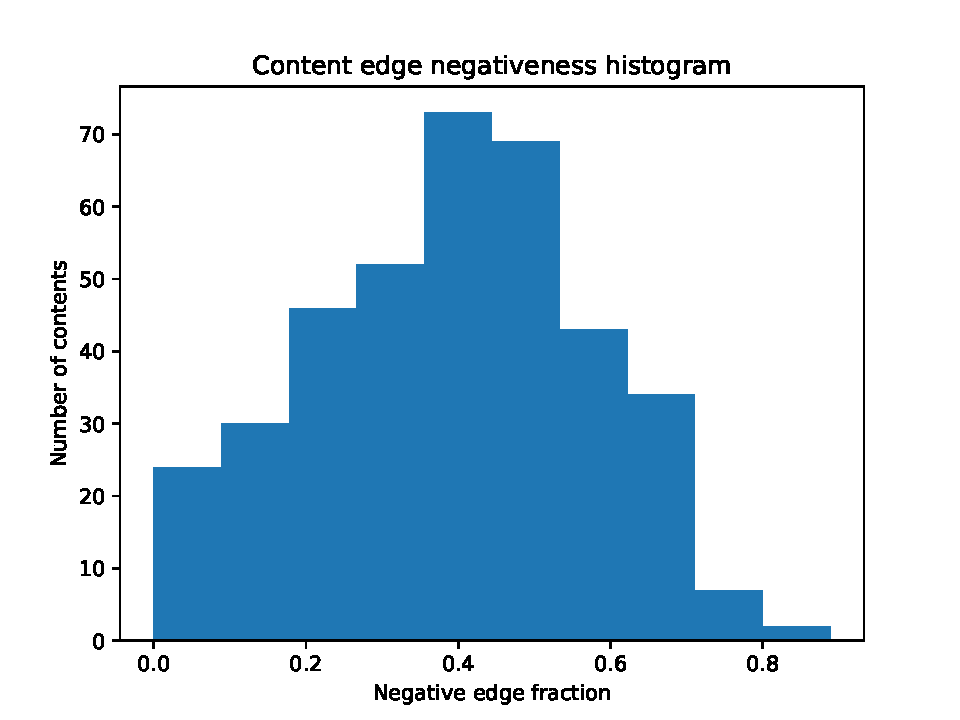
\includegraphics[width=\textwidth]{tex/out/bbcnews500/neg-fraction-content-hist.pdf}
			\caption{$\eta(C)$ of @bbcnews}
			\label{fig:CNN-content-eta}
		\end{subfigure}
		\begin{subfigure}[b]{0.4\textwidth}
			\centering
			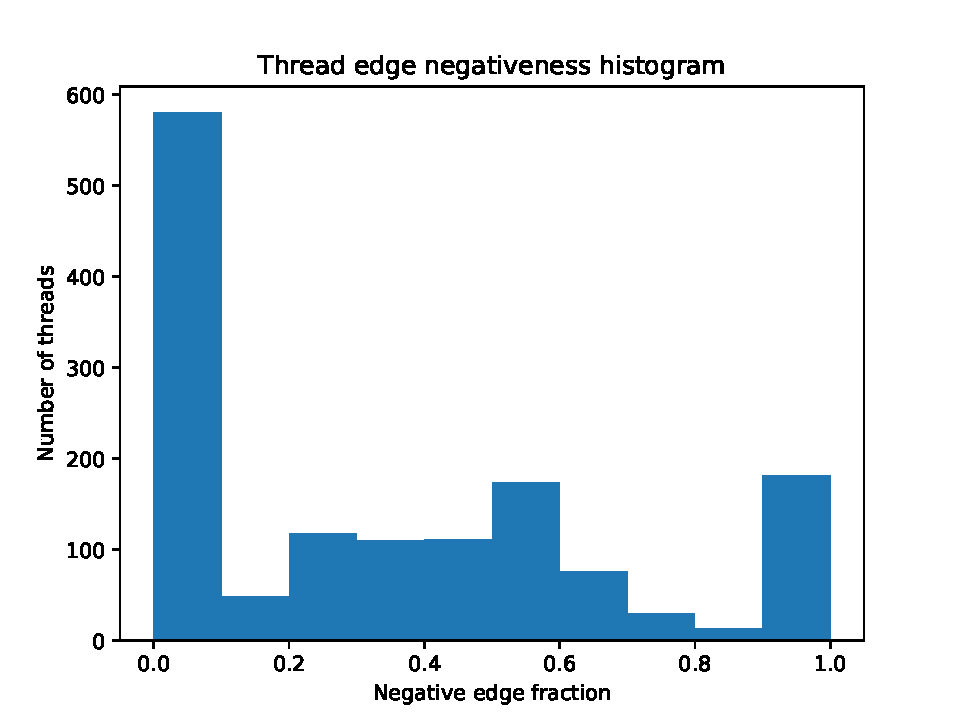
\includegraphics[width=\textwidth]{tex/out/bbcnews500/neg-fraction-thread-hist.pdf}
			\caption{$\eta(T)$ for @bbcnews}
			\label{fig:CNN-thread-eta}
		\end{subfigure}
		\caption{$\eta(C)$ and $\eta(T)$ distribution for many datasets.}
		\label{fig:eta-content-thread}
	\end{center}
\end{figure}

\bigskip
For verifying the reliability of the definition of \emph{controversial}
content,
we also looked at the fraction of negative edges for different datasets, each
associated to contents of the same topic, which we report in
\autoref{tab:eta-subreddits}.

These results show an intuitive association between the fraction of negative edges in the
graph and the topic discussed:
graphs dealing with well-known \emph{controversial} contents, like r/politics and
r/asktrumpsupporters, are the one producing a higher fraction of negative
edges. Also, as expected, they are followed by related topics
(r/economics and r/climate) and football, while
subreddits in which discussions over technologies and sciences
predominate generally have less negative interactions between the users.

\begin{table}
	\centering
	\caption[Fraction of negative edges in different subreddits]{Fraction of negative edges for datasets build on different
		subreddits, each for $200$ contents.}
	\label{tab:eta-subreddits}
	{\small
		\begin{tabular}{|c p{6cm} p{2cm} |}
			\toprule
			Dataset              & Description                               &
			Fraction of neg. edges                                                                       \\
			\midrule
			r/cats               & Pictures and videos about cats            & \num{0.16922540125610608} \\
			r/Covid19            & Scientific discussion of the pandemic     & \num{0.2981398553220806}  \\
			r/programming        & Computer Programming discussions          & \num{0.30264993026499304} \\
			r/climate            & News about climate and related politics   & \num{0.391787072243346}   \\
			r/Football           & News, Rumors, Analysis of \mbox{football} & \num{0.41103067250904934} \\
			r/Economics          & News and discussion about economics       & \num{0.41730200715730514} \\
			r/Politics           & News and discussion about U.S. politics   & \num{0.5112245929821013}  \\
			r/AskTrumpSupporters & {Q\&A between Trump supporters and non
			supporters}          & \num{0.5329949238578681}                                              \\
			\bottomrule
		\end{tabular}
	}
\end{table}

\bigskip
Furthermore, for each content $C$ in an interaction graph, we plotted in
\autoref{fig:edge-sum-n-interactions} the relationship between its number of
interactions and the sum of the weights of its edges.

This relationship is closely related to the $\eta(C)$ of a content: let $E(C)$
be the set of edges associated to content $C \in \mathcal{C} $. We have that
\begin{align*}
	\sum^{}_{e_{ij} \in E(C)} w_{ij} & = \sum^{}_{e_{ij} \in E^+(C)} |w_{ij}|
	- \sum^{}_{e_{ij} \in E^-(C)} |w_{ij}|                                      \\
	                                 & = \sum^{}_{e_{ij} \in E(C)} |w_{ij}| - 2
	\sum^{}_{e_{ij} \in E^-(C)} |w_{ij}|.
\end{align*}

Thus, if we take the ratio with the number of interactions  and suppose
$|w_{ij}| \approx 1$ we obtain
\begin{equation}
	\label{eq:angular-coeff-eta}
	\frac{\sum^{}_{e_{ij} \in E^(C)} |w_{ij}| - 2 \sum^{}_{e_{ij} \in E^-(C)}
	|w_{ij}|}{|E(C)|} \approx 1 - 2 \eta(C).
\end{equation}

\begin{figure}
	\begin{center}
		\begin{subfigure}[b]{0.4\textwidth}
			\centering
			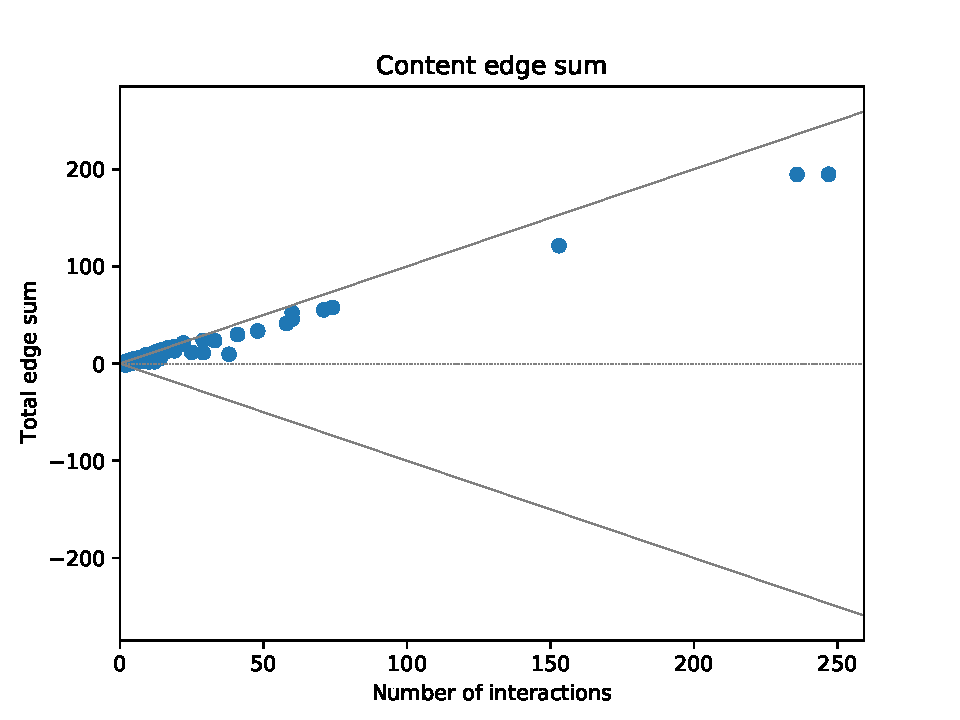
\includegraphics[width=\textwidth]{tex/out/cats200/edge-sum-n-interactions.pdf}
			\caption{r/cats}
			\label{fig:tex/out/cats200/edge-sum-n-interactions.pdf}
		\end{subfigure}
		\begin{subfigure}[b]{0.4\textwidth}
			\centering
			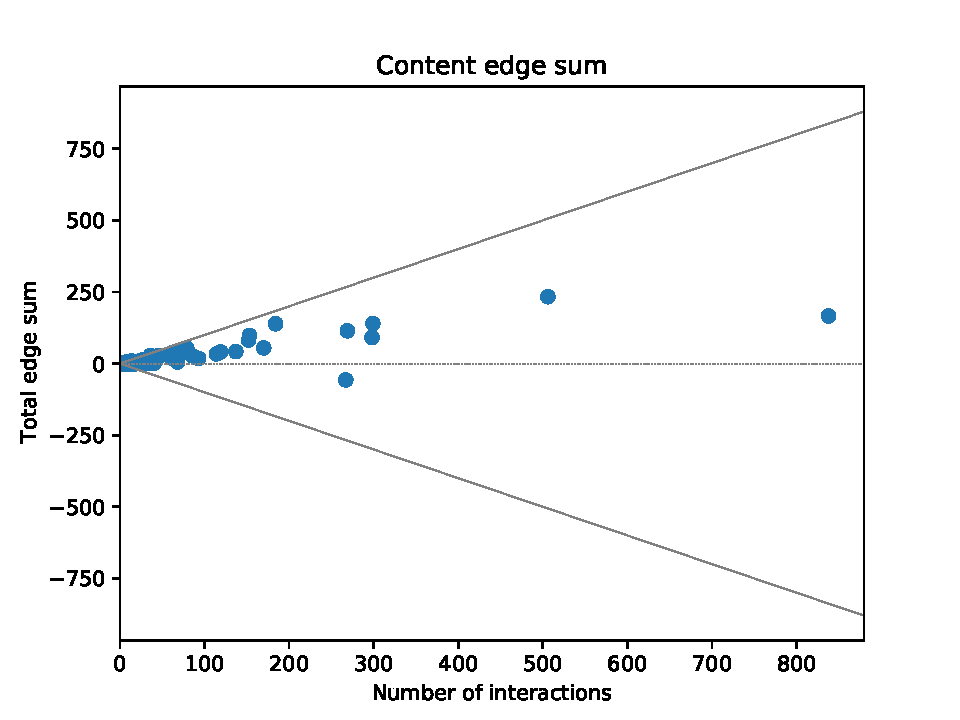
\includegraphics[width=\textwidth]{tex/out/covid19200/edge-sum-n-interactions.pdf}
			\caption{r/covid19}
			\label{fig:tex/out/covid19200/edge-sum-n-interactions.pdf}
		\end{subfigure}
		\begin{subfigure}[b]{0.4\textwidth}
			\centering
			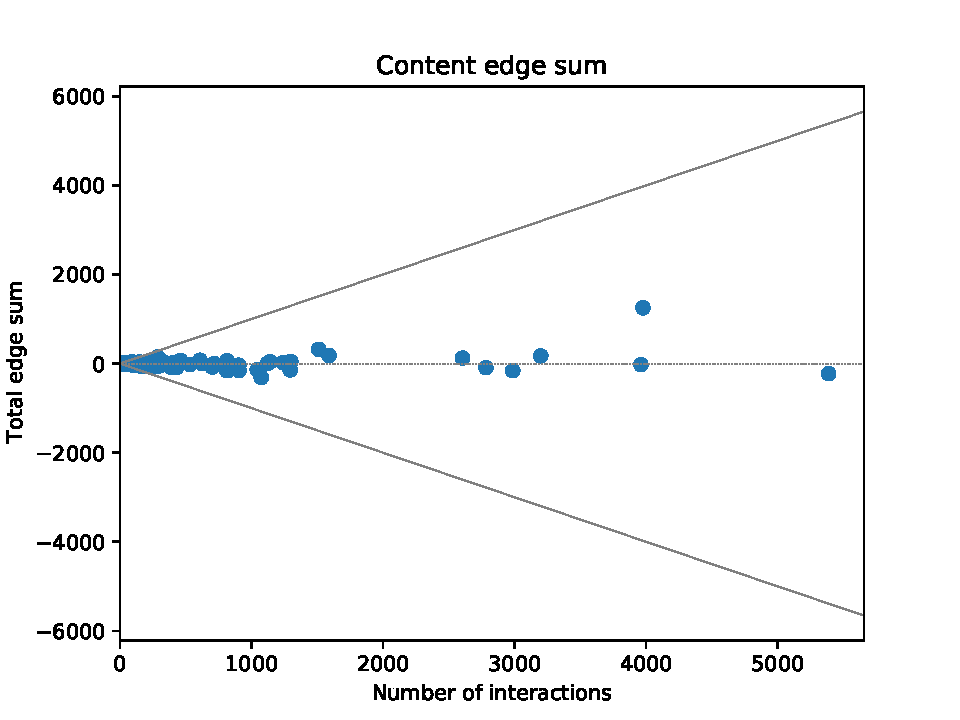
\includegraphics[width=\textwidth]{tex/out/politics200/edge-sum-n-interactions.pdf}
			\caption{r/politics}
			\label{fig:tex/out/politics200/edge-sum-n-interactions.pdf}
		\end{subfigure}
		\begin{subfigure}[b]{0.4\textwidth}
			\centering
			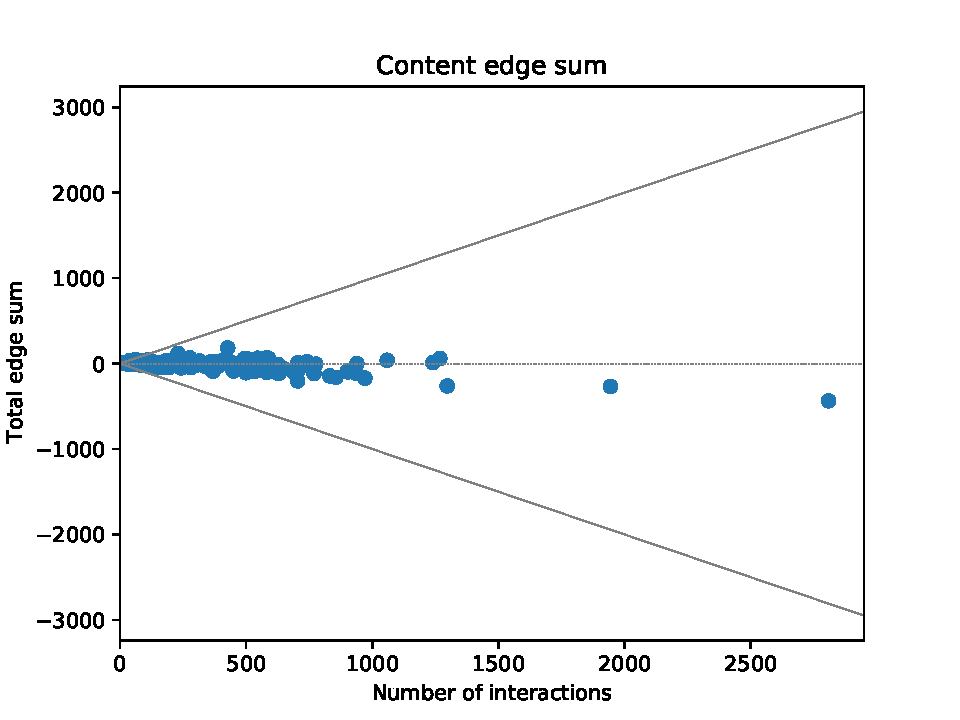
\includegraphics[width=\textwidth]{tex/out/asktrumpsupporters200/edge-sum-n-interactions.pdf}
			\caption{r/asktrumpsupporters}
			\label{fig:tex/out/covid19200/edge-sum-n-interactions.pdf}
		\end{subfigure}
	\end{center}
	\caption[Sum edges over number of interactions for many datasets]{Plots of
		sum of the edges weights over the number of interaction for contents
		from different datasets/subreddits.}
	\label{fig:edge-sum-n-interactions}
\end{figure}

We can see in the plots that content distributes in a pattern which is very
similar to that of a line with rare or no ourliers. Due to
\eqref{eq:angular-coeff-eta} this means that $\eta(C)$ is very similar for
different contents $C$, thus the points create a line whose angular coefficient
is exactly \eqref{eq:angular-coeff-eta}.

Consequently, as we would intuitively say, contents related
to politics are generally controversial, and most of them, as we can see
in \autoref{fig:tex/out/politics200/edge-sum-n-interactions.pdf}, have a high
$\eta(C)$.

This is even more clearly visible when plotting the histogram of $\eta(C)$ for the contents in the dataset
(\autoref{fig:eta-distribution-content}), with most of the contents having a
$\eta(C)$ which is very close to the fraction of negative edges in the graph
reported in \autoref{tab:eta-subreddits}.

\begin{figure}
	\begin{center}
		\begin{subfigure}[b]{0.4\textwidth}
			\centering
			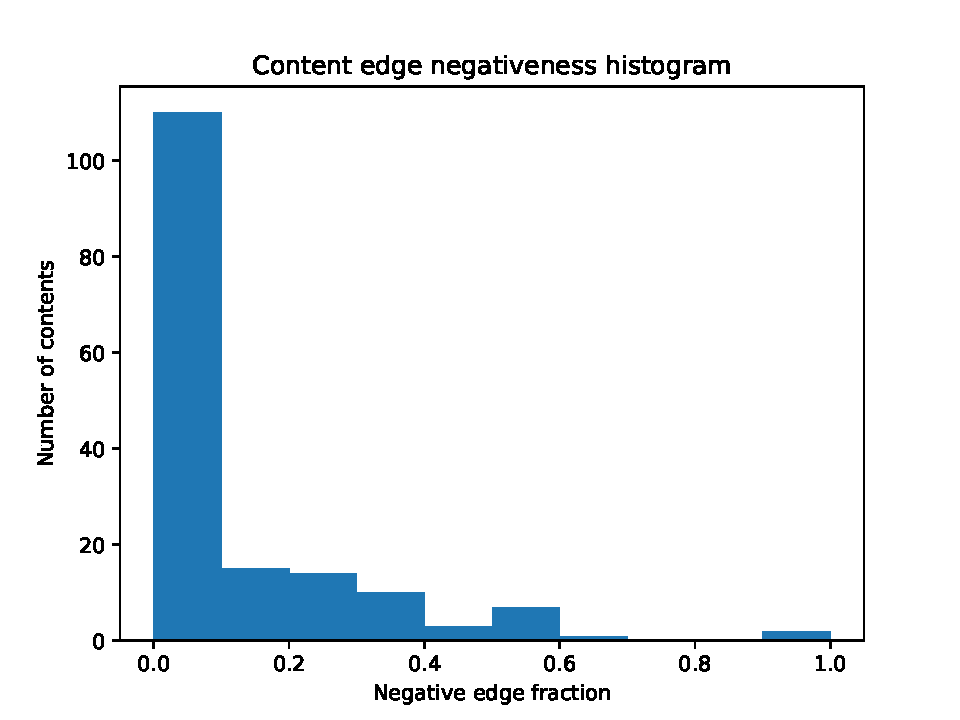
\includegraphics[width=\textwidth]{tex/out/cats200/neg-fraction-content-hist.pdf}
			\caption{r/cats}
			\label{fig:tex/out/cats200/neg-fraction-content-hist.pdf}
		\end{subfigure}
		\begin{subfigure}[b]{0.4\textwidth}
			\centering
			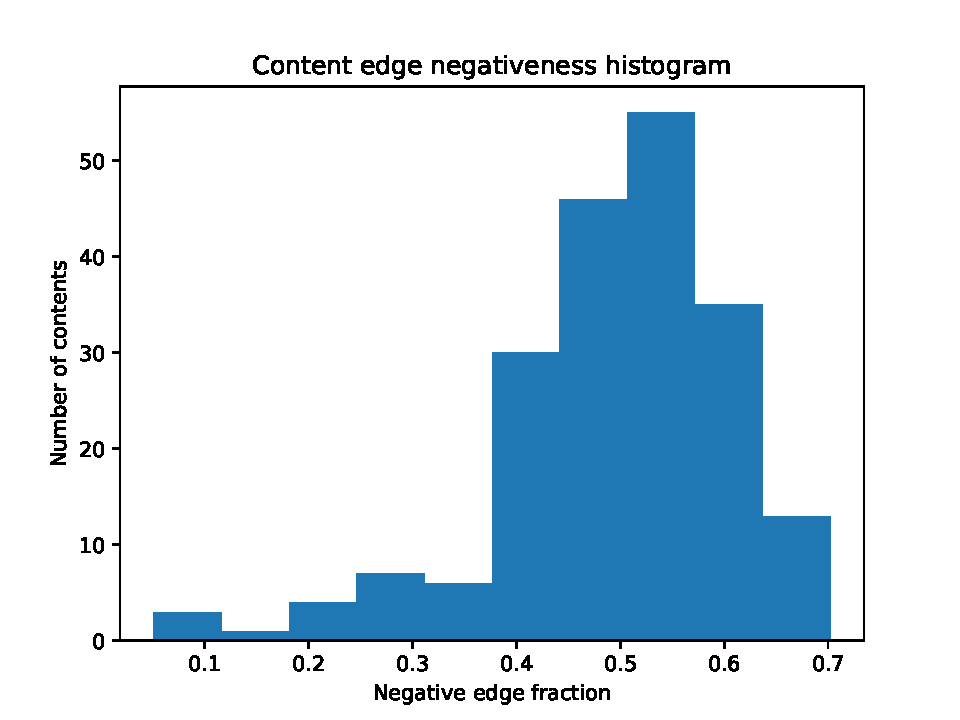
\includegraphics[width=\textwidth]{tex/out/asktrumpsupporters200/neg-fraction-content-hist.pdf}
			\caption{r/asktrumpsupporters}
			\label{fig:asktrump-hist-eta}
		\end{subfigure}
	\end{center}
	\caption{$\eta(C)$ distribution for $2$ of the datasets shown in
		\autoref{fig:edge-sum-n-interactions}.}
	\label{fig:eta-distribution-content}
\end{figure}

\subsection{Tests on synthetic data}%
\label{sub:testing_on_synthetic_data}

For studying how the model behaves in controlled situations we define a
parametrized model based on the Information Spread model
(\autoref{sub:synthetic_data}).

We will generate graphs with four communities, i.e.\ $k= 4$. Also, We choose $\beta _{a} = 1$, meaning that all nodes will be active in each
thread. This a
simplifying assumption which allows us to have a better grasp of the results.
Because of this choice the values $\beta _n = 1$, $\theta = 1$ and
\begin{equation}
	\phi_{rs}  =
	\begin{cases}
		1, \; & \text{if } r = s, \\
		0, \; & \text{otherwise }
	\end{cases} \quad\quad \text{for all } r,s \; groups
\end{equation}
do not influence the structure of the resulting graph.

We also choose $\omega ^{-} _{rs}$ and $\omega ^{+} _{rs} $ to be dependent on
a \emph{noise} variable $x$. More specifically, we choose
\begin{equation}
	\omega_{rs}^{+}   =
	\begin{cases}
		1 - x, \;        & \text{if } r = s, \\
		\frac{x}{4},  \; & \text{otherwise,}
	\end{cases} \quad\quad \text{for all } r,s \; groups
\end{equation}
and
\begin{equation}
	\omega_{rs}^{-}   =
	\begin{cases}
		x, \;                & \text{if } r = s, \\
		\frac{1 - x}{4},  \; & \text{otherwise,}
	\end{cases} \quad\quad \text{for all } r,s \; groups.
\end{equation}

In absence of noise ($x = 0$) we will generate threads whose communities are
positive cliques and all the edges between vertices in different communities
(which will be present with probability $1/4$) are negative.

We will compare different techniques for finding echo chambers (which,
in this case, we will consider as corresponding to a community).

The approach, described in detail in \autoref{alg:clustering_process}, involves calling an algorithm (generally any of the methods presented
in \autoref{ch:solving}) returning a set of users $U \subseteq V$ which will be
labeled according to the majority of its members (by looking at the
ground-truth assignment).
Let $E_k$ be the edges of thread $T_k$. We then remove the edges contributing to $\xi(U)$, i.e\
\begin{equation*}
	\{ e_{ij} \in E_k[U], T_k \in \mathcal{S}_{C}(U), C \in \mathcal{\hat{C}}
	\}.
\end{equation*}
After repeating $k$ times this process, where $k$ is the number
of communities in the model, we compare the ground-truth labels and the
predictions through the Jaccard coefficient and the Adjusted RAND
index\footnotemark.

\begin{algorithm}
	\KwIn{$G = (V, E) \leftarrow $ interaction graph, $\alpha \in [0, 1]$,
		$\mathcal{L} $ ground truth labels of $V$, $\mathcal{I} $ possible
		labels}
	\KwOut{Jaccard and Adjusted RAND index}
	\SetAlgoLined

	// Initialize predicted labels $\mathcal{P} $ with $-1$ (no label)\;
	$\mathcal{P}[v] \leftarrow -1$ for all $v \in V$ \;

	\ForEach{ $i \in \mathcal{I} $ }{
		$U \leftarrow $ solve \acrshort{ECP} on $G$ \;
		// Remove edges contributing to $\xi(U)$ \;
		$E \leftarrow E \setminus \{ e_{ij} \in E_k, T_k \in \mathcal{S}_C(U),
			C \in \mathcal{\hat{C}}\}$ \;

		$l \leftarrow $ majority label of users $U$ in $\mathcal{L} $ \;
		// Do not label again labeled nodes \;
		$U' \leftarrow U \setminus \{ v \in U \; s.t. \; \mathcal{P}[v] \neq -1
			\}$ \;
		$\mathcal{P}[v] = l $ for all $v \in U'$ \;
	}

	// Compute Jaccard for each label and take the average \;
	$J[l] \leftarrow Jaccard( \{ v \in V \; s.t. \; \mathcal{P}[v] = l \}, \; \{ v \in
		V\; s.t. \; \mathcal{L}[v] = l \})  $ for each $l \in \mathcal{I} $ \;
	Jaccard score $\leftarrow \sum^{}_{l \in \mathcal{I} } J[l] / |\mathcal{I}|  $ \;
	Adjusted RAND index $\leftarrow $ Adjusted RAND($\mathcal{P} $, $\mathcal{L} $)
	\;

	\Return Jaccard score, Adjusted RAND index\;
	\caption{Clustering process}
	\label{alg:clustering_process}
\end{algorithm}

\footnotetext{The Adjusted RAND index is a measure of similarity between
	different clusterings. It is based on the RAND index, which compares
	the number of agreeing pairs in the $2$ solutions; the Adjusted one corrects
	the RAND Index "by chance", i.e. compares it to the expected index
	(i.e.\ of a random assignment). For more details we
	refer to \cite{CharuC.Aggarwal2013}.}

What we expect is that, as the value of $x$ increases, the produced threads
will have generally more negative edges inside a community and more positive
edges between different communities, making it more difficult for our
algorithms to find the set of vertices corresponding to one of the Echo
Chambers.

\begin{figure}
	\begin{center}
		\begin{subfigure}[b]{0.4\textwidth}
			\centering
			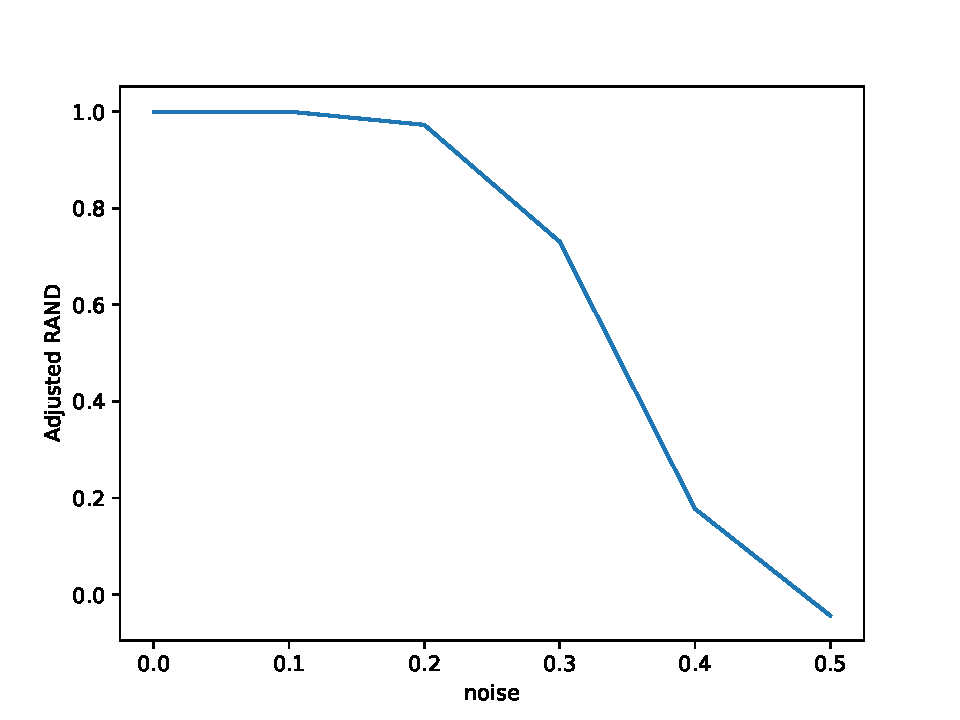
\includegraphics[width=\textwidth]{tex/out/synthetic_exact/model2_noise_adj_rand.pdf}
			\caption{Adjusted RAND index, MIP}
			\label{fig:tex/out/synthetic_exact/model2_noise_adj_rand.pdf}
		\end{subfigure}
		\quad
		\begin{subfigure}[b]{0.4\textwidth}
			\centering
			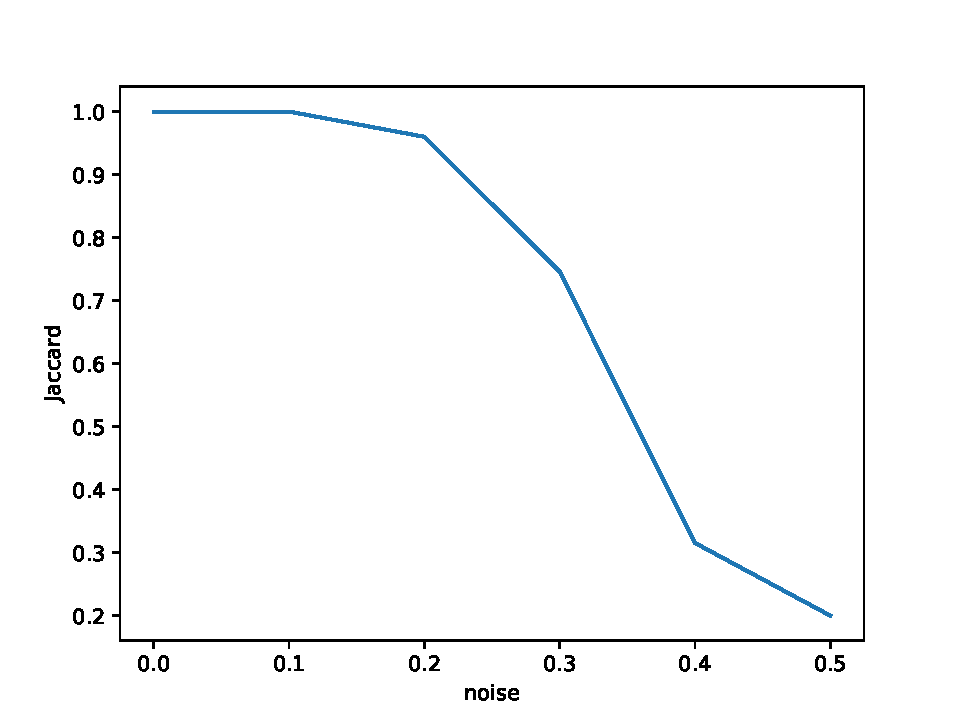
\includegraphics[width=\textwidth]{tex/out/synthetic_exact/model2_noise_jaccard.pdf}
			\caption{Jaccard Score, MIP}
			\label{fig:tex/out/synthetic_exact/_noise_jaccard.pdf}
		\end{subfigure}
		\begin{subfigure}[b]{0.4\textwidth}
			\centering
			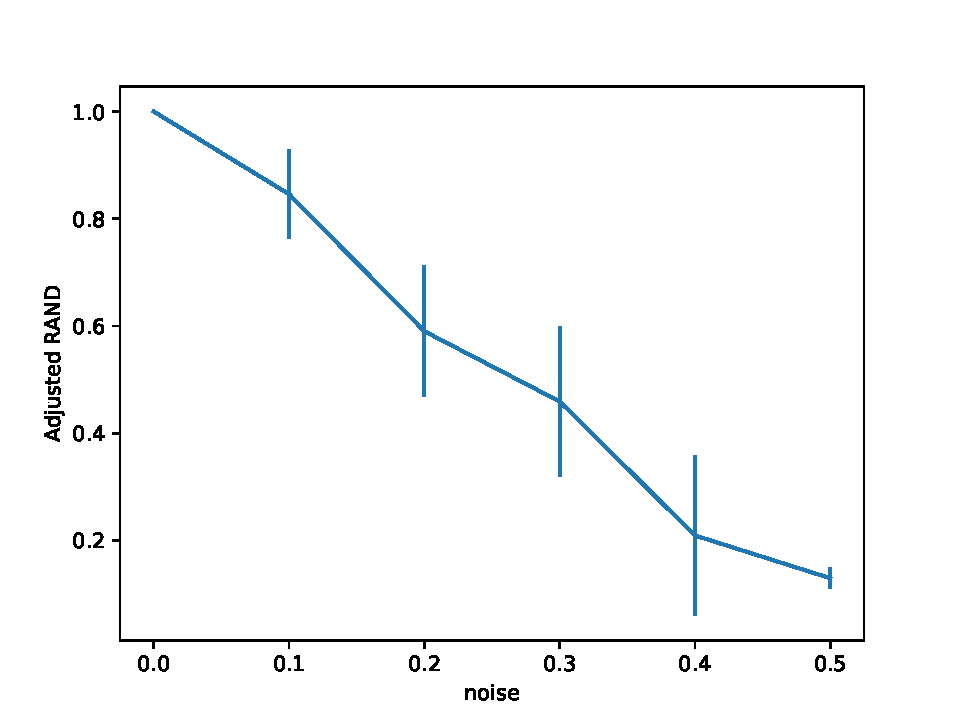
\includegraphics[width=\textwidth]{tex/out/synthetic_12t/model2_noise_adj_rand.pdf}
			\caption{Adjusted RAND index, \mbox{rounding algorithm}}
			\label{fig:tex/out/synthetic_exact/model2_noise_adj_rand.pdf}
		\end{subfigure}
		\quad
		\begin{subfigure}[b]{0.4\textwidth}
			\centering
			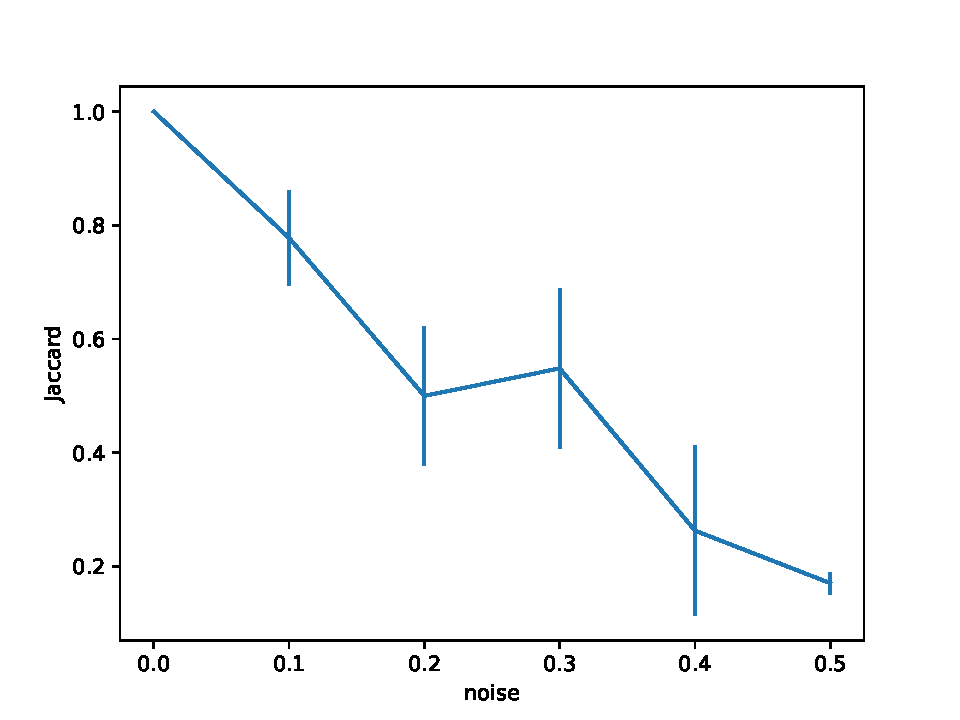
\includegraphics[width=\textwidth]{tex/out/synthetic_12t/model2_noise_jaccard.pdf}
			\caption{Jaccard Score, \mbox{rounding algorithm}}
			\label{fig:tex/out/synthetic_exact/_noise_jaccard.pdf}
		\end{subfigure}
	\end{center}
	\caption{Clustering scores on generated graphs with 12 threads and four communities, each
		of six nodes, for different values of the noise
		variable~$x$.}
	\label{fig:clustering-mip-rounding}
\end{figure}

We compared the scores obtained with the \acrshort{MIP} for the \acrshort{ECP}
(\autoref{sub:a_mip_model_for_the_ecp}) and the Rounding algorithm
(\autoref{sub:approximation_algorithms}). Due to the use of the
\acrshort{MIP} model these experiments have been carried out on
small graphs with four communities, each of six nodes. The interaction graph
contains 12 threads and we choose $\alpha = 0.2$. We experimentally saw that
this choice of parameters produces controversial contents, thus allowing our
methods to be applied.

Note that since we choose $\alpha = 0.2$ our analysis is partially limited for $x
	> 0.2$ since we may produce graphs that have a fraction of negative
\emph{intra-community} edges
higher than $\alpha $, although it is smaller than the fraction of negative
\emph{inter-community} edges. Nonetheless, we may be able to reconstruct at least
partially the communities.

The performances of the two approaches are shown in
\autoref{fig:clustering-mip-rounding}. We can see that the MIP model
\begin{itemize}
	\item Reconstructs perfectly the communities for values of $x \in \{0,
		      0.1\}$.
	\item Predicts almost perfectly the labels for $x= 0.2$.
	\item Reconstructs partially the communities for $x = 0.3$, achieving both
	      a Jaccard coefficient and an Adjusted RAND Index around $0.7$.
	\item Fails to find the original groups of users for $x \geq 0.4$.
\end{itemize}

The MIP formulation is generally better at finding the communities since, if
the noise $x$ is not too large, the best score is still achieved
by selecting mostly nodes in the same community (choosing nodes from other
communities will generally add many more negative edges to the subgraph).

Conversely, the rounding algorithm is more affected by noise than MIP. More
specifically, the rounding algorithm:
\begin{itemize}
	\item Reconstructs the communities perfectly for values of $x = 0$.
	\item Partially recognizes the communities for $x= 0.1$, obtaining a
	      Jaccard coefficient and Adjusted RAND Index around $0.8$.
	\item Finds few users belonging to the same community for $x = 0.2$, with
	      scores around $0.6$.
	\item Fails to find the original groups of users for $x \geq 0.3$.
\end{itemize}
We illustrate its limitations with one example. Consider the graph in
\autoref{fig:rounding-interaction-graph-example} for $\alpha = 0.1$:
the MIP model will find one of the two communities as optimal solution.
Now consider the rounding algorithm (\autoref{sub:approximation_algorithms}):
the relaxation of the MIP will assign to all positive edges value
$0.66$, while the negative edges get value $0$. This means that the algorithm
will initially iterate over the positive edges, choosing randomly among them (since they have the same value).
We illustrate in \autoref{fig:rounding-run-unlucky} one possible iteration: in
this case the algorithm will not be able to reconstruct one of the communities
exactly since the considered edge will not allow the heuristic to have a single component of
$\hat{G}$ associated to one of the communities.
Conversely, in \autoref{fig:rounding-run-lucky} we can see a "luckier"
iteration in which it is able to find one of the communities.

More generally, we can say that the rounding algorithm is less robust to noise
than the MIP, especially if the noise produces an increase in the number of
positive \emph{inter-community} edges, as we saw in the example of
\autoref{fig:rounding-example}.

This is due to the fact that it may need to pick among positive edges with the
same value (in the solution of the relaxation) during its execution: if the picked edge connects different communities, this will most
likely prevent the algorithm from having communities as separate component in
the dummy graph $\hat{G}$ (\autoref{sub:approximation_algorithms}).

% This is due to the fact that the rounding algorithm performances depends on the
% probability of picking these positive
% \emph{inter-community} edges (the lower the probability is, the higher the
% chances of a correct clustering).

% Consequently, we can expect than if we decrease the number of these positive
% \emph{inter-community} edges with respect to the number of positive
% \emph{intra-community}, the algorithm is more likely to reconstruct correctly
% the Echo Chambers.

Consequently, we could improve the performances of the algorithm by decreasing the probability
of picking inter-community edges, or, equivalently, increasing the probability
of picking intra-community edges. For example, we could increase the latter probability
by rising the number of threads in an interaction graph.

We repeated this experiment with a different number of threads
while maintaining the same set of parameters as before. We show the results
obtained by the rounding algorithm in \autoref{fig:clustering-threads}: we obtain better clustering
performances as the number of threads increases, especially for values of
$x \in \{ 0.0, 0.1 \}$.

\begin{figure}
	\begin{center}
		\begin{subfigure}{0.3\textwidth}
			\centering
			\tikzfig{tex/tikz/rounding_original}
			\caption{An example of interaction graph $G$}
			\label{fig:rounding-interaction-graph-example}
		\end{subfigure}
		\quad
		\begin{subfigure}{0.3\textwidth}
			\centering
			\tikzfig{tex/tikz/rounding_exec}
			\caption{A possible state of $\hat{G}$ when running the rounding
				algorithm}
			\label{fig:rounding-run-unlucky}
		\end{subfigure}
		\quad
		\begin{subfigure}{0.3\textwidth}
			\centering
			\tikzfig{tex/tikz/rounding_exec_lucky}
			\caption{Another possible state of $\hat{G}$ when running the
				rounding algorithm}
			\label{fig:rounding-run-lucky}
		\end{subfigure}
	\end{center}
	\caption[An interaction graph with a single thread and content and two
		possible iterations of the rounding algorithm]{Possible rounding algorithm
		executions on an interaction graph with a
		one thread and one content. The two communities are represented by $\{ v_1, v_2,
			v_3\}$ and $\{ v_4, v_5, v_6\}$, respectively. Negative and
		positive edges are coloured in red and green, respectively.
		For $\alpha = 0.1$ we will have that its content is
		controversial and the exact solution returns either one of
		the two communities. The rounding algorithm may fail to reconstruct
		communities if the edge between the communities ($e_{35}$) is added early in
		the iterations (\autoref{fig:rounding-run-unlucky}).}
	\label{fig:rounding-example}
\end{figure}

\begin{figure}
	\begin{center}
		\begin{subfigure}[b]{0.3\textwidth}
			\centering
			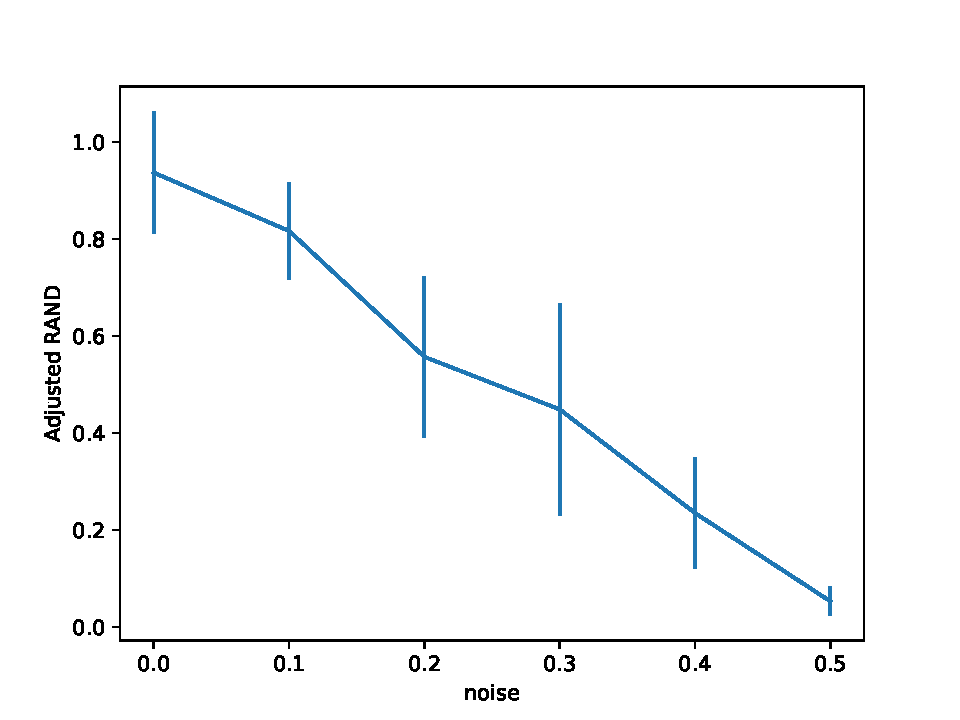
\includegraphics[width=\textwidth]{tex/out/synthetic_8t/model2_noise_adj_rand.pdf}
			\caption{8 threads}
			\label{fig:tex/out/synthetic_8t/model2_noise_adj_rand.pdf}
		\end{subfigure}
		\begin{subfigure}[b]{0.3\textwidth}
			\centering
			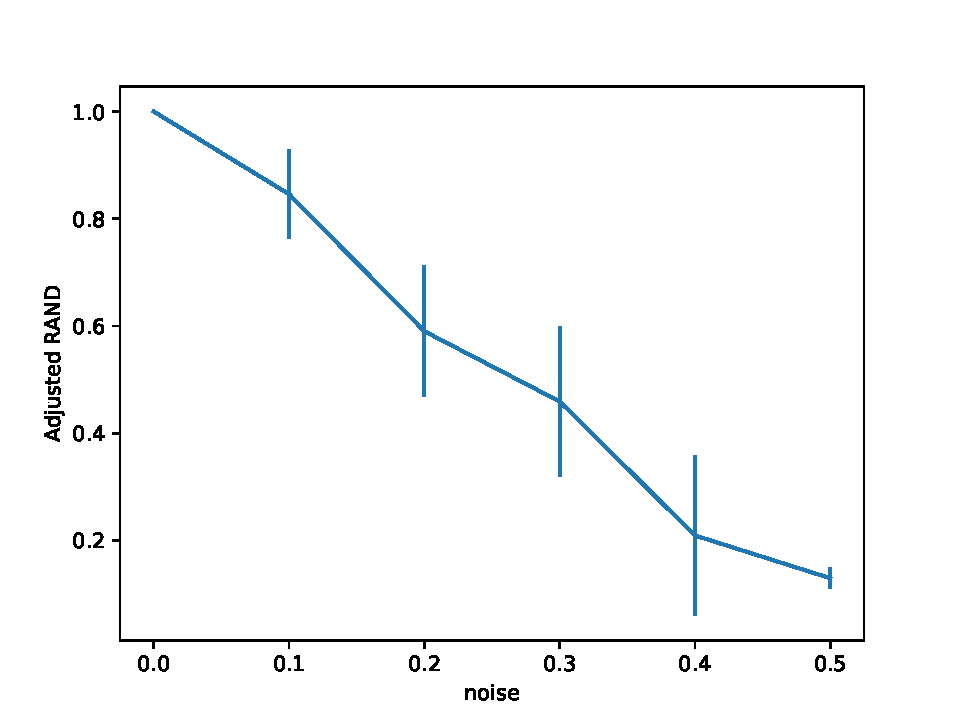
\includegraphics[width=\textwidth]{tex/out/synthetic_12t/model2_noise_adj_rand.pdf}
			\caption{12 threads}
			\label{fig:tex/out/synthetic_8t/model2_noise_adj_rand.pdf}
		\end{subfigure}
		\begin{subfigure}[b]{0.3\textwidth}
			\centering
			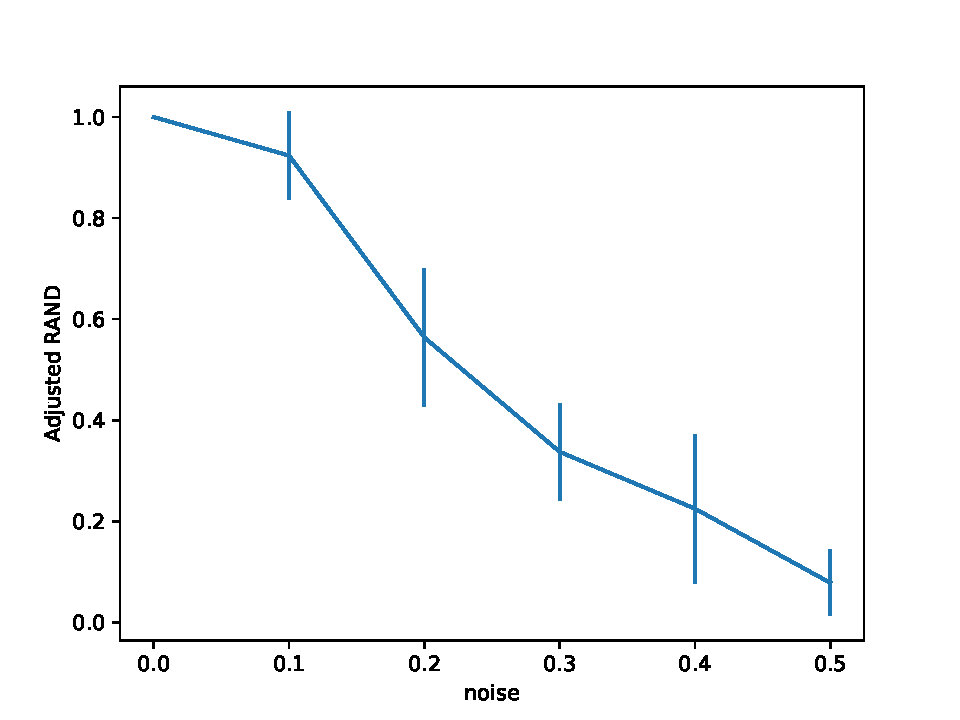
\includegraphics[width=\textwidth]{tex/out/synthetic_20t/model2_noise_adj_rand.pdf}
			\caption{20 threads}
			\label{fig:tex/out/synthetic_8t/model2_noise_adj_rand.pdf}
		\end{subfigure}
	\end{center}
	\caption{Adjusted RAND indices for graphs with four communities, each of
		six nodes, and different number of threads, obtained with the rounding
		algorithm.}
	\label{fig:clustering-threads}
\end{figure}

\subsection{Detecting real-world echo chambers}%
\label{sub:detecting_real_echo_chambers}

We measured the performances of the rounding algorithm on real-world data by
classifying the nodes of labeled datasets, similarly to what has been done
with synthetic data. Recall from \autoref{sec:data_collection_and_generation},
that for these datasets we have retrieved a label for each user.

We will refer to a group of users with the same label as \emph{community}.

We ran the experiments on the r/asktrumpsupporters and
@nytimes datasets. In the first case users label themselves either as Trump Supporters ($19\%$), Non
Supporters ($79\%$) or Undecided ($2\%$). This last group of users was ignored
in the analysis, i.e.\ these vertices were removed from the graph.

In the @nytimes dataset users are labeled either as democrats ($80\%$) or republican
($20\%$). In this case, in order to decrease the sparsity, we selected the
$4$-core.

% Both of them are unbalanced datasets, with r/asktrumpsupporters having a
% and  of the users choosing the \emph{Non Supporter} and \emph{Trump
%     Supporter} flairs, respectively (the remaining  is
% \emph{Undecided}), while  of @nytimes users are labeled \emph{democrats}
% and  as \emph{republican}.

We cluster the nodes as shown in \autoref{alg:clustering_process}
and choose $\alpha $ as the median of the $\eta(C), C \in \mathcal{C} $. We run
the rounding algorithm to find the Echo Chambers. By
looking at the poor results, which we show in
\autoref{tab:scores-datasets-labeled}, it is clear that the algorithm is not
able to correctly separate the communities. We motivate this with the following
reasons:
\begin{itemize}
	\item \textbf{Non-validity of the data model.} In trying to classify the
	      nodes with our \acrshort{ECP} solver, we are assuming that the data
	      contains a clear separation of the users, in which one chamber
	      corresponds to a single community. Furthermore, we are assuming that
	      there are only two communities in the datasets we chose, which may also
	      be a limiting assumption, since:
	      \begin{itemize}
		      \item @nytimes may contain echo chambers related to different
		            topics, as the set of contents does not only take into account
		            U.S. political discussions.
		      \item r/asktrumpsupporters may be a non-representative
		            dataset of discussion of polarized communities (we
		            discuss this more in details in
		            \autoref{sec:the_r_asktrumpsupporters_case}).
	      \end{itemize}
	\item \textbf{Complexity of sentiment analysis of social media language.}
	      Social medias often involve messages which are not easily classifiable
	      as either friendly and hostile, both because users often use jargon
	      and because sometimes messages are aided by pictures and GIFs which
	      are not taken into account by the sentiment analyzer.
	      % additional noise is introduced by messages in other languages as well
	      % as messages involving medias like pictures and GIF.
	\item \textbf{Limitations of the rounding algorithm.} Since we are
	      using an approximation algorithm we are not solving exactly the
	      \acrshort{ECP}: this may introduce limitations to the solutions which
	      is used to cluster the nodes. More specifically, since at each iteration it uses a set of users
	      connected by positive edges as possible solution (see
	      \autoref{ssub:rounding_algorithm}), it is likely to return
	      a set $U$ with just one connected component.
	\item \textbf{Sparsity of the data}. We can see from
	      \autoref{tab:scores-datasets-labeled} that the two datasets are
	      sparse.
	      This, as we discussed in \autoref{sub:testing_on_synthetic_data}, is
	      important factor in achieving good performances, especially for the
	      rounding algorithm.
	      More generally, this is a limitation of real-world data:
	      we observed, especially on Twitter, that even increasing the number of
	      contents does not produce denser graphs, as the average degree remains
	      between one and two.
	      Furthermore, analyzing the $k$-core, a denser part of the graph, may
	      affect the results since we expect that the echo chamber effect is
	      especially visible in small and isolated components, maybe a small
	      "bubble" of users sharing the same opinion, which may get excluded by
	      the $k$-core selection.

\end{itemize}

\begin{table}
	\centering
	\caption{Classification scores obtained with the
		rounding algorithm on two labeled datasets. $\alpha $ is chosen as the
		median $\eta(C)$, $C \in
			\mathcal{C} $. For the @nytimes dataset we report the statistics
		related to its $4$-core. $|\{T\}|$ indicates the number of threads.}
	\label{tab:scores-datasets-labeled}
	{\small
		\begin{tabular}{|ccccc p{1.8cm} c|}
			\toprule
			Dataset              & $|V|$         & $|E|$                     & $|\mathcal{C}| $          &
			$|\{T\}| $           & Adjusted RAND & Jaccard                                                                                                            \\
			\midrule
			r/asktrumpsupporters & 11640         & 83038                     & 357
			                     & 357           & \num{0.09453599837921367} & \num{0.01607717041800643}                                                              \\
			@nytimes             & 1074          & 4921                      & 139                       & 254 & \num{0.02176064966494696} & \num{0.4200626959247649} \\
			\bottomrule
		\end{tabular}
	}
\end{table}

\section{Further discussion of the results}%
\label{sec:discussion}

We focused our experiments on the rounding algorithm. We did this
since we observed that, when running the other heuristic algorithms on smaller datasets
(with less than $3000$ nodes), its \emph{time} performances were generally better
than those of the peeling algorithm (\autoref{sub:approximation_algorithms}).
Also, when compared to the $\beta$-approach, the rounding algorithm is more
expressive: we already discussed in \autoref{sub:approximation_algorithms} that
the $\beta$-approach is able to find only group of nodes that are connected.

We report in \autoref{tab:times-approximation} the execution times on some
datasets. While execution \emph{times} of the peeling approach explode with
@BBCTech and r/cats, the rounding algorithm and the $\beta $-approach show a
more stable trend, with most of the experiments of both of them being completed
in less than $6$ seconds.

\begin{table}
	\centering
	\caption[Execution time of the heuristics]{Execution time in seconds of
		the heuristics. Here, $\alpha$ is chosen to be the median of the
		$\eta(C)$ for each dataset.}
	\label{tab:times-approximation}
	\begin{tabular}{c|c|c|c|c|c}
		Dataset         & $|V|$ & $|E|$ & Rounding                 & Peeling                  & $\beta$                  \\
		\hline
		@EMA\_News      & 1226  & 1842  & \num{0.9331817626953125} & \num{24.05003571510315}  & \num{36.05760359764099}  \\
		@bbcsciencenews & 447   & 388   & \num{4.916658878326416}  & \num{175.36006140708923} & \num{0.7964000701904297} \\
		% @BBCSport       & 2140 & 3100 &                          &                          &                          \\
		@BBCNewsEnts    & 220   & 183   & \num{4.617515325546265}  & \num{138.2591540813446}  & \num{0.4381392002105713} \\
		@BBCTech        & 793   & 719   & \num{86.20259594917297}  & \num{2798.376838684082}  & \num{0.9822568893432617} \\
		r/cats          & 2493  & 4028  & \num{5.439620494842529}  & \num{140844.752099514}   & \num{0.7333328723907471} \\
		% r/covid19                &                          &                         &                          &         &         \\
	\end{tabular}
\end{table}

% Similarly, due to evident complexity limitations we were able to execute the exact
% \acrshort{MIP} only on very small synthetic datasets, as shown in
% \autoref{sub:synthetic_data}.
\bigskip

We summarize our results for the rounding algorithm as follows. It achieves good performances on data with
polarized communities, showing also to be more robust as the
available data increases: a larger number of threads, as we discussed
in \autoref{sub:testing_on_synthetic_data}, helps the algorithm selecting
\emph{intra-community} edges, which allows it to correctly classify the nodes.
Conversely, the rounding algorithm was not able to produce a good clustering of the
nodes in real-world data.
